% !TEX root = progress-llncs.tex
\newcommand{\PREAMBLE}

\section{Example: A Signal Control System}
\label{sec:example}

We illustrate our method by applying it to design a system controlling
trains at a
station~\cite{hudon11:_devel_contr_system_guided_model_envir}.  We
first present some informal requirements of the system.

\subsection{Requirements}
\label{sec:requirements}

\begin{wrapfigure}{r}{0.55\linewidth}
  \centering \ifx\PREAMBLE\UnDef
\documentclass{beamer}
\usepackage{tikz}
\usetikzlibrary{snakes,arrows}

\usepackage[english]{babel}
% or whatever

\usepackage[latin1]{inputenc}
% or whatever

\usepackage[T1]{fontenc}
\usepackage{amssymb}
\usepackage{amsmath}
\usepackage{eventB}

\begin{document}
\else
\fi


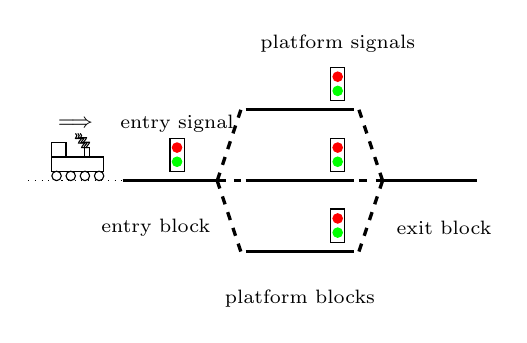
\begin{tikzpicture}[scale=0.6]
  \scriptsize
  % approaching block.
  \draw[very thick] (0,0) -- (1.5,0);
  \draw (0.7, -1) node{entry block};

  % in-switch
  \draw[very thick] (1.5,0) -- (2,0);
  \draw[very thick, dashed] (2,0) -- (2.5,1.5);
  \draw[very thick, dashed] (2,0) -- (2.5,-1.5);
  \draw[very thick, dashed] (2,0) -- (2.5,0);
%  \draw[red] (2, -1.5) node{in-switch};
  
  % platform blocks
  \draw[very thick] (2.6,0) -- (4.9,0);
%  \draw[very thick, dotted] (2.6,0.5) -- (4.9,0.5);
%  \draw[very thick, dotted] (2.6,-0.5) -- (4.9,-0.5);
  \draw[very thick] (2.6,1.5) -- (4.9,1.5);
  \draw[very thick] (2.6,-1.5) -- (4.9,-1.5);
  \draw (3.75, -2.5) node{platform blocks};

  % out-switch
  \draw[very thick] (5.5,0) -- (6,0);
  \draw[very thick, dashed] (5,1.5) -- (5.5,0);
  \draw[very thick, dashed] (5,0) -- (5.5,0);
  \draw[ very thick, dashed] (5,-1.5) -- (5.5,0);
%  \draw[red] (5.5, -1.5) node{out-switch};

  % exiting block.
  \draw[very thick] (6.0,0) -- (7.5,0);
  \draw (6.8, -1) node{exit block};

  % entry signal
%  \draw[very thick] (1.45,0) -- (1.45, 1);
  \draw (1, 0.2) rectangle +(0.3,0.7);
  \filldraw[red] (1.15, 0.7) circle (0.1);
  \filldraw[green] (1.15, 0.4) circle (0.1);
  \draw (1.15, 1.2) node{entry signal};

  % platform signals
%  \draw[very thick] (6.05,0) -- (6.05, 1);
  \draw (4.4, 0.2) rectangle +(0.3,0.7);
  \filldraw[red] (4.55, 0.7) circle (0.1);
  \filldraw[green] (4.55, 0.4) circle (0.1);
  \draw (4.55, 2.9) node{platform signals};

  \draw (4.4, 1.7) rectangle +(0.3,0.7);
  \filldraw[red] (4.55, 2.2) circle (0.1);
  \filldraw[green] (4.55, 1.9) circle (0.1);

  \draw (4.4, -1.3) rectangle +(0.3,0.7);
  \filldraw[red] (4.55, -0.8) circle (0.1);
  \filldraw[green] (4.55, -1.1) circle (0.1);

  % The train
  \draw[dotted] (-2,0) -- (0, 0);
  \draw(-1.5,0.2) rectangle +(1.1, 0.3);
  \draw(-1.5,0.5) rectangle +(0.3, 0.3);
  \draw(-0.8,0.5) rectangle +(0.1, 0.2);
  \draw[decorate, decoration={snake, amplitude = 1pt, segment length = 2pt}] (-0.8,0.7) --  (-1,1);
  \draw[decorate, decoration={snake, amplitude = 1pt, segment length = 2pt}] (-0.75,0.7) --  (-0.95,1);
  \draw[decorate, decoration={snake, amplitude = 1pt, segment length = 2pt}] (-0.7,0.7) --  (-0.9,1);
  \draw (-1.4, 0.1) circle (0.1);
  \draw (-1.1, 0.1) circle (0.1);
  \draw (-0.8, 0.1) circle (0.1);
  \draw (-0.5, 0.1) circle (0.1);
  \draw (-1, 1.2) node{$\Longrightarrow$};
\end{tikzpicture}

\ifx\PREAMBLE\UnDef
\end{document}
\else
\fi

  \caption{A signal control system}
  \label{fig:sgnctrl}
\end{wrapfigure}

The network at the station contains an \emph{entry block}, several
\emph{platform blocks} and an \emph{exiting block}, as seen in
Figure~\ref{fig:sgnctrl}.  Trains arrive on the network at the entry
block, then can move into one of the platform blocks before moving to
the exiting block and leaving the network (see Figure~\ref{fig:sgnctrl}).
% \begin{requirements}
%   \asm{asm:topology}{There is one entry block, many platform blocks and
%     one exiting block, connected together as shown in
%     Figure~\ref{fig:sgnctrl}.}
%   \asm{asm:movement}{Trains travel in one direction from the entry block
%     to the exiting block via a platform block}
% \end{requirements}
In order to control the trains at the station, signals are positioned
at the end of the entry block and each platform block.  The
train drivers are assumed to obey the signals.  The signals are
supposed to change from green to red automatically when a train passes by.
% \begin{requirements}
%   \asm{asm:entry-signal}{There is a light signal at the end of
%     the entry block}\ReqSpacing
%   \asm{asm:platform-signal}{There is a light signal at the end of each
%     platform block}\ReqSpacing
%   \asm{asm:obey-signal}{Trains obey the light signals} \ReqSpacing
%   \asm{asm:signal-to-red}{Signals change from green to red
%     automatically when a train passes by}
% \end{requirements}

The most important properties of the system are that (1) there should be
no collision between trains (\ref{saf:no-collision}), and (2) each train in the network eventually
leaves~(\ref{live:train-leave}).
\begin{requirements}
  \saf{saf:no-collision}{There is at most one train on each block}\ReqSpacing
  \req{live:train-leave}{Each train in the network eventually leaves}
\end{requirements}

\paragraph{Refinement strategy} In the initial model, we abstractly
model the trains in the network, focusing on~\ref{live:train-leave}.
In the first refinement, we introduce the topology of the network.  We
strengthen the model of the system, focusing on~\ref{saf:no-collision}
in the second refinement.  In the third refinement, we introduce the
signals and derive a specification for the controller that manages
these signals.
% As one can see, the liveness requirement, i.e.,
% \ref{live:train-leave}, is taken early in the development and acts as
% a guideline for designing the system.

\subsection{Initial Model}
\label{sec:initial-model}
\newBset[TRAIN]{TRN}
\newBvrb[trains]{trns}
\newBpar[train]{t}
\newBevt{arrive}
\newBevt{depart}
\newBinv[invTrainType]{inv0\_1}

In this initial model, we use a carrier set \TRAIN to denote the set of
trains and a variable \trains to denote the set of trains currently
within the network.  Initially \trains is assigned the empty set.  At
this abstract level, we have two events to model a train arriving at
the station and a train leaving the station as below.
\begin{Bcode}
  % $
  % \variables{\trains}
  % $
  % \Bhspace
  % $
  % \invariants{\invTrainType: & \trains \subseteq \TRAIN}
  % $
  % \Bvspace
  % $
  % \initialisation{\trains \bcmeq \emptyset}
  % $
  % \Bvspace
  $
  \ubeventinline{\arrive}
  {\train}
  {\train \in \TRAIN}
  {}
  {}
  {\trains \bcmeq \trains \bunion \{\train\}}
  $
  \Bhspace
  $
  \ubeventinline{\depart}{\train}{\train \in \TRAIN}{}{}{\trains \bcmeq
    \trains \setminus \{\train\}}
  $
\end{Bcode}

The requirement \ref{live:train-leave} can be specified as a progress
property \Binv{prg0\_1}: $ \train \in \trains \leadsto t \notin
\trains$.  According to \eqref{eq:trans-prop}, \Binv{prg0\_1} is
equivalent to \Binv{prg0\_2}: $\tr \train \in \trains$.  In order to
implement this transient property, we rely on
Theorem~\ref{thm:transient} and add scheduling information for event
\depart as follows.
\begin{Bcode}
  $
  \ubeventinline{\depart}{\train}{\train \in \TRAIN}{\train \in \trains}{}{\trains \bcmeq \trains \setminus \{\train\}}
  $
\end{Bcode}
Here, we design our \depart event to implement the transient property
\Binv{prg0\_2} such that conditions \eqref{eq:SCH} and \eqref{eq:OP}
are trivial.  For condition \eqref{eq:NEG}, it is easy to prove that
\depart establishes the fact $\train \notin \trains$ in one
step.

Since event \arrive will not affect our reasoning about progress
properties (it is always unscheduled), we are going to omit the
refinement of \arrive in the subsequent presentation.

\subsection{First Refinement}
\label{sec:first-refinement}

\newBset[BLOCK]{BLK}
\newBcst{Entry}
\newBcst[PLATFORM]{PLF}
\newBcst{Exit}
\newBaxm[axmBlockType]{axm1\_1}
\newBvrb[location]{loc}
\newBinv[invLocationType]{inv1\_1}
\newBevt{moveout}
\newBevt{movein}

In this refinement, we first introduce the topology of the network
in terms of blocks.  We introduce a carrier set \BLOCK and three
constants \Entry, \PLATFORM, \Exit denoting the entry block, platform
blocks and exit block, respectively.
% \begin{Bcode}
% $
% \axioms[false]{
%   \axmBlockType: & \partition(\BLOCK, \{Entry\}, \PLATFORM, \{Exit\})
% }
% $
% \end{Bcode}
A new variable \location is introduced denoting the location of trains
in the network, constrained by invariant \invLocationType: $\location
\in \trains \tfun \BLOCK$.
% We refine event \arrive to state that the train to arrive at the entry
% block.
% \begin{Bcode}
%   $
%   \ubevent{\arrive}{\train}{\train \notin \trains}{}{}{
%     \ldots \\
%     \location(\train) \bcmeq \Entry
%   }
%   $
% \end{Bcode}

For event \depart, we strengthen the guard to state that a train can
only leave from the exit block.  Subsequently, in order to make sure
that the schedule is stronger than the guard~(condition
\eqref{eq:fis}), we need to strengthen the coarse-schedule
accordingly (see Figure~\ref{fig:1st-ref}).
In order to prove the refinement of \depart, we apply
Theorem~\ref{thm:ref-rep-crs} (coarse-schedule replacing).  In
particular we need to prove the following conditions:
\begin{gather}
  \train \in \trains ~\leadsto~ \train \in \trains
  \land \location.\train = \Exit \label{eq:33}
  \tag{\Binv{prg1\_1}} \\
  \train \in \trains \land \location.\train =
    \Exit ~\un~ \spneg (\train \in \trains) \label{eq:34}
  \tag{\Binv{un1\_2}}
\end{gather}

\begin{figure}[!hbtp]
  \centering
  \begin{Bcode}[\scriptsize]
    $ \ubevent{\depart}{\train}{ \train \in \trains \land
      \location.\train = \Exit } { \train \in \trains \land
      \location.\train = \Exit} {} {\trains \bcmeq \trains \setminus
      \{\train\} \\ \location \bcmeq \{\train\} \domsub \location} $
    \Bhspace[0.1em]
    $
  \ubevent{\moveout}{\train}
  {\train \in \trains \land \location.\train \in \PLATFORM}
  {\train \in \trains \land \location.\train \in \PLATFORM}
  {}
  {\location.\train \bcmeq \Exit}
  $
  \Bhspace[0.1em]
  $
  \ubevent{\movein}{\train}
  {\train \in \trains \land \location.\train = \Entry}
  {\train \in \trains \land \location.\train = \Entry}
  {}
  {\location \bcmsuch \qexists{p}{p \in \PLATFORM}{\location'
    = \location \ovl \{\train \mapsto p\}}}
  $
  \end{Bcode}
  \vspace{-4ex}
  \caption{Events of the first refinement}
  \label{fig:1st-ref}
\end{figure}

From now on, we focus on reasoning about progress properties, e.g.,
\ref{eq:33}, omitting the reasoning about unless properties, e.g.,
\ref{eq:34}.  The readers should be convinced that using
Theorem~\ref{thm:unless}, these unless properties are valid for our
model.  We first apply \eqref{eq:37} to obtain $\train \in \trains
\land \location.\train \neq \Exit ~\leadsto~ \train \in \trains \land
\location.\train = \Exit$ and then apply the transitivity
property~\eqref{eq:transitivity} of the leads-to operator to establish
two progress properties \ref{eq:24} and \ref{eq:25} as follows.
\begin{gather}
  \label{eq:24}
  \train \in \trains \land \location.\train
  \neq \Exit ~\leadsto~ \train \in
  \trains \land \location.\train \in \PLATFORM
  \tag{\Binv{prg1\_3}}\\
  \label{eq:25}
  \train \in \trains \land \location.\train
  \in \PLATFORM ~\leadsto~ \train \in
  \trains \land \location.\train = \Exit
  \tag{\Binv{prg1\_4}}
\end{gather}
Consider \ref{eq:25}, we first apply the ensure-rule
(Theorem~\ref{thm:ensure-rule}) to establish two properties (after
simplification) as follows:
\begin{gather}
  \label{eq:27}
  \train \in \trains \land \location.\train \in \PLATFORM ~\un~
  \train \in \trains \land \location.\train = \Exit
  \tag{\Binv{un1\_5}}\\
  \label{eq:28}
  \tr \train \in \trains \land \location.\train \in
    \PLATFORM
  \tag{\Binv{prg1\_6}}
\end{gather}

We apply Theorem~\ref{thm:transient} to implement \ref{eq:28} by the
new event \moveout which has a weakly-fair scheduling (see
Figure~\ref{fig:1st-ref}).
% \begin{Bcode}[\footnotesize]
%   $
%   \ubevent{\moveout}{\train}
%   {\train \in \trains \land \location.\train \in \PLATFORM}
%   {\train \in \trains \land \location.\train \in \PLATFORM}
%   {}
%   {\location.\train \bcmeq \Exit}
%   $
% \end{Bcode}
The proof that \moveout implements \ref{eq:28} is straightforward and
therefore is omitted.

Similarly, for \ref{eq:24}, we apply the ensure-rule and implementing
the resulting transient property, i.e., $\tr \train \in \trains \land
\location.\train = \Entry$, by event \movein in Figure~\ref{fig:1st-ref}.
%  The first condition first is equivalent to
% \begin{Bcode}
%     $ \train \in \trains \land
%     \location(\train) \neq \Exit \land
%     \location(\train) \notin \PLATFORM ~\leadsto~ \train \in
%   \trains \land \location(\train) \in \PLATFORM $
% \end{Bcode}

% \begin{Bcode}
%     $ \train \in \trains \land
%     \location(\train) = \Entry ~\leadsto~ \train \in
%   \trains \land \location(\train) \in \PLATFORM $
% \end{Bcode}
% applies the ensure rule
% \begin{Bcode}
%   $\train \in \trains \land
%   \location(\train) = \Entry ~\un~ \train \in
%   \trains \land \location(train) \in \PLATFORM $
%   \\
%   $\tr \train \in \trains \land \location(\train) = \Entry \land \neg (\train \in
%   \trains \land \location(\train) \in \PLATFORM)$
% \end{Bcode}
% The transient property can be implemented by the following event
% \begin{Bcode}[\footnotesize]
%   $
%   \ubevent{\movein}{\train}
%   {\train \in \trains \land \location.\train = \Entry}
%   {\train \in \trains \land \location.\train = \Entry}
%   {}
%   {\location \bcmsuch \qexists{p}{p \in \PLATFORM}{\location'
%     = \location \ovl \{\train \mapsto p\}}}
%   $
% \end{Bcode}

% Currently, our model includes the requirements about the topology
% of the network and the possible movement of trains within the network,
% i.e., \ref{asm:topology} and \ref{asm:movement}.

\subsection{Second Refinement}
\label{sec:second-refinement}
In this refinement, we incorporate the safety requirement stating that
there are no collisions between trains within the network,
i.e. \ref{saf:no-collision}.  This is captured by invariant
\Binv{inv2\_1} about \location: $\qforall{\train_1,\train_2}{\train_1, \train_2 \in \trains \land \location.\train_1 =
  \location.\train_2}{\train_1 = \train_2}$.
% Safety: No collision is model by injectivity property of \location.
% \begin{Bcode}
%   $
%   \invariants{
%     \location \in \trains \pinj \BLOCK
%   }
%   $
% \end{Bcode}
% Event \arrive is refined straightforward
% \begin{Bcode}
%   $
%   \ubevent{\arrive}{\train}{\train \notin \trains \\ \Entry \notin \ran(\location) }{}{}{
%     \trains \bcmeq \trains \bunion \{\train\} \\
%     \location(\train) \bcmeq \Entry
%   }
%   $
% \end{Bcode}

The guard of event \moveout needs to be strengthened to maintain
\Binv{inv2\_1}.  As a result, we need to modify the schedule
information to ensure the \emph{feasibility} condition~\eqref{eq:fis}
for \unitb events stating that the schedules are stronger than the
guard.  In particular, we add (strengthen) the fine-schedule of
\moveout (see Figure~\ref{fig:2nd-ref}).
\begin{figure}[!htbp]
  \centering
  \begin{Bcode}[\scriptsize]
    $ \ubevent{\moveout}{\train}{ \train \in \trains \land
      \location.\train \in \PLATFORM \land \\
      \Exit \notin \ran.\location
    }{\train \in \trains \land \location.\train \in \PLATFORM} {\Exit
      \notin \ran.\location} {\location.\train \bcmeq \Exit} $
    \Bhspace
  $
  \ubevent{\movein}{\train}
  {\train \in \trains \land \location.\train = \Entry \land
    \qexists{p}{p \in \PLATFORM}{p \notin \ran.\location}
  }
  {\train \in \trains \land \location.\train = \Entry  \land     \qexists{p}{p \in \PLATFORM}{p \notin \ran.\location}}
  {}
  {\location \bcmsuch \qexists{p}{p \in \PLATFORM \setminus 
    \ran.\location}{\location'
    = \location \ovl \{\train \mapsto p\}}}
  $
  \end{Bcode}
  \vspace{-4ex}
  \caption{Events of the second refinement}
  \label{fig:2nd-ref}
\end{figure}
The scheduling information for \moveout states that for any train
$\train$, if $\train$ stays in a platform for infinitely long and the
exit block becomes free infinitely often, then $\train$ can move out of the
platform.

%\marginpar{Simon: Rephrase this paragraph if possible}
We want to highlight the fact that \moveout has both a coarse- and a
fine-schedule.  In particular, using only either weak- or
strong-fairness would be unsatisfactory.
Weak-fairness requires for the exit block to be remain free continuously in order for
trains to move out.  This assumption is not met by the current system.
Strong-fairness allows a train to leave if the train is present on the
platform intermittently.  This assumption is more flexible than we
need since it allows behaviours where a train hops on and off
the platform infinitely often. The price of that flexibility is to entangle 
properties of the exit block with properties of trains: indeed, we would
need not only to prove that the train will be on its platform and that 
the exit block will become free but that both happen simultaneously
infinitely often.

%\todo{Son: (to SImon) We need to make this point clearer. What I want
%  to focus here is that coarse-/fine-schedules are suitable
%  specification rather than weak-/strong-fairness.}
We choose to relinquish this flexibility and are therefore capable of structuring
our proof better: on one hand, the train stays on its platform as
long as necessary; independently, the exit block becomes free
infinitely many times. 

In order to prove the refinement of \moveout, we apply
Theorem~\ref{thm:strengthen-fns} (fine-schedule strengthening), which
requires to prove the following progress property (remember that when
an event has no fine schedules, it is assumed to be $\one$).
\begin{equation}
  \label{eq:31}
  \one \leadsto \Exit \notin \ran.\location
  \tag{\Binv{prg2\_3}}
\end{equation}
Property
\ref{eq:31} is equivalent to transient property \Binv{prg2\_4}: $\tr
\Exit \in \ran.\location$.  We satisfy \Binv{prg2\_4} by applying the
transient rule (Theorem~\ref{thm:transient}) using event \depart where
the value for the parameter $\train$ is given by
$\location^{-1}.\Exit$, i.e., the train at the exit block.  The
proofs of conditions~\eqref{eq:SCH}, \eqref{eq:OP}, and \eqref{eq:NEG} are
straight-forward.

Finally we strengthen the guard of \movein and subsequently strengthen
its coarse-schedule (see Figure~\ref{fig:2nd-ref}).  We apply
Theorem~\ref{thm:ref-rep-crs} (coarse-schedule replacing) \movein.
The detailed proof is omitted here.

\subsection{Third Refinement}
\label{sec:third-refinement}

\newBset{COLOR}
\newBcst[GREEN]{GR}
\newBcst[RED]{RD}
\newBvrb[signal]{sgn}
\newBevt[ctrlplf]{ctrl\_platform}
\newBpar[platform]{p}

In this refinement, we introduce the signals associated with different
blocks within the network.  Variable \signal is introduced to denote
the value of the signals associated with different blocks.  We focus
on the controlling of the platform signals here.  In particular,
invariants \Binv{inv3\_2} and \Binv{inv3\_3} state that if a platform signal is
green (\GREEN) then the exit block is free and the other platform
signals are red (\RED).
  \begin{Bcode}[\footnotesize]
    $ \invariants[false]{ \Binv{inv3\_1}: & \signal \in \{\Entry\}
      \bunion \PLATFORM \tfun
      \COLOR \\
      \Binv{inv3\_2}: & \qforall{p}{p \in \PLATFORM \land \signal.p =
        \GREEN}{\Exit \notin \ran.\location} \\
      \Binv{inv3\_3}: & \qforall{p,q}{p, q \in \PLATFORM \land
        \signal.p = \signal.q = \GREEN}{p = q} } $
  \end{Bcode}

\begin{figure}[!htbp]
  \centering
  \begin{Bcode}[\scriptsize]
    $
    \ubevent{\moveout}{\train}{
      \train \in \trains \land
      \location.\train \in \PLATFORM \land \\
      \signal.(\location.\train) = \GREEN
    }{\train \in \trains \land \location.train \in \PLATFORM \land \\
    \signal.(\location.\train) = \GREEN}{}{\location.\train \bcmeq
    \Exit \\
    \signal.(\location.\train) \bcmeq \RED
  }
  $
  \Bhspace
  $
  \ubevent{\ctrlplf}{\platform}{
    \platform \in \PLATFORM \land
    \platform \in \ran.\location \land
    \Exit \notin \ran.\location \land \\
    \qforall{q}{q \in \PLATFORM}{\signal.q = \RED}
  }
  {
    \platform \in \PLATFORM \land
    \platform \in \ran.\location \land
    \signal.\platform = \RED
  }
  {
    \Exit \notin \ran(\location) \land
    \qforall{q}{q \in \PLATFORM \land q \neq \platform}{\signal.q = \RED}
  }
  {\signal.\platform \bcmeq \GREEN}
  $
\end{Bcode}
\vspace{-4ex}
\caption{Events of the third refinement}
\label{fig:3rd-ref}
\end{figure}
We refine the \moveout event using the platform signal as shown in Figure~\ref{fig:3rd-ref}.
The refinement of \moveout is justified by applying
Theorem~\ref{thm:ref-rep-crs} (coarse-schedule replacing) and
Theorem~\ref{thm:remove-fns} (fine-schedule removing).  In particular,
replacing the coarse-schedule requires the following progress
property.
\begin{equation}
  \label{eq:99}
  \train \in \trains \land \location.\train \in \PLATFORM
  \wide\leadsto \train \in \trains \land \location.\train \in
  \PLATFORM \land \signal.(\location.\train) = \GREEN
  \tag{\Binv{prg3\_4}}
\end{equation}
which can be implemented by
\begin{equation}
  \label{eq:35}
  \tr \train \in \trains \land \location.\train \in
  \PLATFORM \land \signal.(\location.\train) = \RED~.
  \tag{\Binv{prg3\_5}}
\end{equation}

In order to satisfy \ref{eq:35}, we introduce a new event
\ctrlplf for the controller to change a platform signal to green according to
Theorem~\ref{thm:transient} (see Figure~\ref{fig:3rd-ref}).
% \begin{Bcode}[\footnotesize]
%   $
%   \ubevent{\ctrlplf}{\platform}{
%     \platform \in \PLATFORM \land
%     \platform \in \ran.\location \land
%     \Exit \notin \ran.\location \land
%     \qforall{q}{q \in \PLATFORM}{\signal.q = \RED}
%   }
%   {
%     \platform \in \PLATFORM \land
%     \platform \in \ran.\location \land
%     \signal.\platform = \RED
%   }
%   {
%     \Exit \notin \ran(\location) \land
%     \qforall{q}{q \in \PLATFORM \land q \neq \platform}{\signal.q = \RED}
%   }
%   {\signal.\platform \bcmeq \GREEN}
%   $
% \end{Bcode}
This event \ctrlplf is a specification for the system to control the
platform signals preserving both safety and liveness properties of the
system.  In particular, the scheduling information states that if (1)
a platform is occupied and the platform signal is \RED infinitely long
and (2) the exit block is unoccupied and the other platform signals
are all \RED infinitely often, then the system should eventually set
this platform signal to \GREEN.

The refinement of event \movein and how the entry signal is controlled
is similar and omitted.

%%% Local Variables: 
%%% mode: latex
%%% TeX-master: "progress"
%%% End: 
